\chapter{Benchmarks}

\section{Queries' execution times}
\begin{table}[h]
	\centering
	\begin{tabular}{|l|>{\ttfamily}r|>{\ttfamily}r|>{\ttfamily}r|}
		\hline
		Algorithm & \normalfont\textbf{AVG [ms]} & \normalfont\textbf{STD DEV [ms]} & \normalfont\textbf{MAX [ms]} \\
		\hline
		DAAT & 25.88 & 19.69 & 78.68 \\
		BMM & 6.67 & 6.29 & 42.48 \\
		\hline
	\end{tabular}
	\caption{Execution times in milliseconds for different algorithms}
	\label{tab:algorithm_times}
\end{table}

\begin{figure}[H]
	\centering
	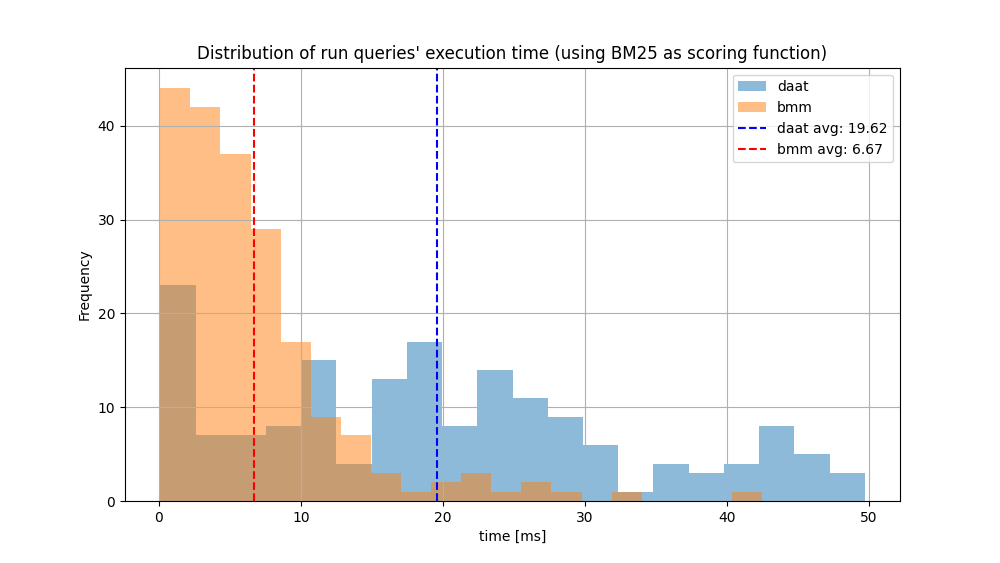
\includegraphics[width=1\textwidth]{assets/times_distrib.png}
	\caption{Distribution of times}
	\label{fig:time_distribution}
\end{figure}

\section{trec\_eval}
\begin{table}[H]
	\centering
	\begin{tabular}{|l|>{\ttfamily}r|>{\ttfamily}r|>{\ttfamily}r|}
		\hline
		Metric & \normalfont\textbf{DAAT} & \normalfont\textbf{BMM} & \normalfont\textbf{Chang's} \\
		\hline
		mAP & 0.1982 & 0.1709 & 0.0794 \\
		RR & 0.8110 & 0.7141 & 0.7285 \\
		ndcg & 0.3376 & 0.2902 & 0.1681\\
		ndcg@10 & 0.4750 & 0.4110 & 0.4075 \\
		ndcg@20 & 0.4705 & 0.4013 & - \\
		set P & 0.4815 & 0.4065  & 0.5163 \\
		set R & 0.2600 & 0.2315 & 0.0987 \\
		set F & 0.2781 & 0.2411 & 0.1437 \\
		\hline
	\end{tabular}
	\caption{trec\_eval for DAAT and BMM}
	\label{tab:metric_comparison}
\end{table}

	\section{Time statistics}
\lstinputlisting[caption={Indexing program's output: it takes less than 1 minute and 20 seconds to build it}, label={lst:example_output}]{assets/build time.txt}

\section{files' size}

\begin{table}[H]
	\centering
	\begin{tabular}{|l|*{5}{c|}c|}
		\hline
		& \textbf{Partition 0} & \textbf{Partition 1} & \textbf{Partition 2} & \textbf{Partition 3} & \textbf{Partition 4} & \textbf{Total} \\
		\hline
		Document Index & 46 & 47 & 46 & 46 & 17 & \textbf{202} \\
		Local Lexicon & 22 & 23 & 23 & 23 & 12 & \textbf{103} \\
		Posting Lists & 131.5 & 174.5 & 174.5 & 173.5 & 61.7 & \textbf{715.7} \\
		\hline
		\multicolumn{6}{|c|}{Global Lexicon} & \textbf{14} \\
		\hline
		\multicolumn{6}{|c|}{\textbf{TOTAL}} & \textbf{1034.7} \\
		\hline
	\end{tabular}
	\caption{Files' sizes, figures in megabytes}
	\label{tab:spanning_table}
\end{table}

\lstinputlisting[caption={Files tree}, label={lst:tree}]{assets/files sizes.txt}

\section{Conclusion and limitations}
